% Options for packages loaded elsewhere
\PassOptionsToPackage{unicode}{hyperref}
\PassOptionsToPackage{hyphens}{url}
\PassOptionsToPackage{dvipsnames,svgnames,x11names}{xcolor}
%
\documentclass[
  super,
  preprint,
  3p]{elsarticle}

\usepackage{amsmath,amssymb}
\usepackage{iftex}
\ifPDFTeX
  \usepackage[T1]{fontenc}
  \usepackage[utf8]{inputenc}
  \usepackage{textcomp} % provide euro and other symbols
\else % if luatex or xetex
  \usepackage{unicode-math}
  \defaultfontfeatures{Scale=MatchLowercase}
  \defaultfontfeatures[\rmfamily]{Ligatures=TeX,Scale=1}
\fi
\usepackage{lmodern}
\ifPDFTeX\else  
    % xetex/luatex font selection
\fi
% Use upquote if available, for straight quotes in verbatim environments
\IfFileExists{upquote.sty}{\usepackage{upquote}}{}
\IfFileExists{microtype.sty}{% use microtype if available
  \usepackage[]{microtype}
  \UseMicrotypeSet[protrusion]{basicmath} % disable protrusion for tt fonts
}{}
\makeatletter
\@ifundefined{KOMAClassName}{% if non-KOMA class
  \IfFileExists{parskip.sty}{%
    \usepackage{parskip}
  }{% else
    \setlength{\parindent}{0pt}
    \setlength{\parskip}{6pt plus 2pt minus 1pt}}
}{% if KOMA class
  \KOMAoptions{parskip=half}}
\makeatother
\usepackage{xcolor}
\setlength{\emergencystretch}{3em} % prevent overfull lines
\setcounter{secnumdepth}{5}
% Make \paragraph and \subparagraph free-standing
\ifx\paragraph\undefined\else
  \let\oldparagraph\paragraph
  \renewcommand{\paragraph}[1]{\oldparagraph{#1}\mbox{}}
\fi
\ifx\subparagraph\undefined\else
  \let\oldsubparagraph\subparagraph
  \renewcommand{\subparagraph}[1]{\oldsubparagraph{#1}\mbox{}}
\fi


\providecommand{\tightlist}{%
  \setlength{\itemsep}{0pt}\setlength{\parskip}{0pt}}\usepackage{longtable,booktabs,array}
\usepackage{calc} % for calculating minipage widths
% Correct order of tables after \paragraph or \subparagraph
\usepackage{etoolbox}
\makeatletter
\patchcmd\longtable{\par}{\if@noskipsec\mbox{}\fi\par}{}{}
\makeatother
% Allow footnotes in longtable head/foot
\IfFileExists{footnotehyper.sty}{\usepackage{footnotehyper}}{\usepackage{footnote}}
\makesavenoteenv{longtable}
\usepackage{graphicx}
\makeatletter
\def\maxwidth{\ifdim\Gin@nat@width>\linewidth\linewidth\else\Gin@nat@width\fi}
\def\maxheight{\ifdim\Gin@nat@height>\textheight\textheight\else\Gin@nat@height\fi}
\makeatother
% Scale images if necessary, so that they will not overflow the page
% margins by default, and it is still possible to overwrite the defaults
% using explicit options in \includegraphics[width, height, ...]{}
\setkeys{Gin}{width=\maxwidth,height=\maxheight,keepaspectratio}
% Set default figure placement to htbp
\makeatletter
\def\fps@figure{htbp}
\makeatother

\usepackage{booktabs}
\usepackage{longtable}
\usepackage{array}
\usepackage{multirow}
\usepackage{wrapfig}
\usepackage{float}
\usepackage{colortbl}
\usepackage{pdflscape}
\usepackage{tabu}
\usepackage{threeparttable}
\usepackage{threeparttablex}
\usepackage[normalem]{ulem}
\usepackage{makecell}
\usepackage{xcolor}
\makeatletter
\makeatother
\makeatletter
\makeatother
\makeatletter
\@ifpackageloaded{caption}{}{\usepackage{caption}}
\AtBeginDocument{%
\ifdefined\contentsname
  \renewcommand*\contentsname{Table of contents}
\else
  \newcommand\contentsname{Table of contents}
\fi
\ifdefined\listfigurename
  \renewcommand*\listfigurename{List of Figures}
\else
  \newcommand\listfigurename{List of Figures}
\fi
\ifdefined\listtablename
  \renewcommand*\listtablename{List of Tables}
\else
  \newcommand\listtablename{List of Tables}
\fi
\ifdefined\figurename
  \renewcommand*\figurename{Figure}
\else
  \newcommand\figurename{Figure}
\fi
\ifdefined\tablename
  \renewcommand*\tablename{Table}
\else
  \newcommand\tablename{Table}
\fi
}
\@ifpackageloaded{float}{}{\usepackage{float}}
\floatstyle{ruled}
\@ifundefined{c@chapter}{\newfloat{codelisting}{h}{lop}}{\newfloat{codelisting}{h}{lop}[chapter]}
\floatname{codelisting}{Listing}
\newcommand*\listoflistings{\listof{codelisting}{List of Listings}}
\makeatother
\makeatletter
\@ifpackageloaded{caption}{}{\usepackage{caption}}
\@ifpackageloaded{subcaption}{}{\usepackage{subcaption}}
\makeatother
\makeatletter
\@ifpackageloaded{tcolorbox}{}{\usepackage[skins,breakable]{tcolorbox}}
\makeatother
\makeatletter
\@ifundefined{shadecolor}{\definecolor{shadecolor}{rgb}{.97, .97, .97}}
\makeatother
\makeatletter
\makeatother
\makeatletter
\makeatother
\journal{Journal of Economic Behavior and Organization}
\ifLuaTeX
  \usepackage{selnolig}  % disable illegal ligatures
\fi
\usepackage[]{natbib}
\bibliographystyle{elsarticle-num}
\IfFileExists{bookmark.sty}{\usepackage{bookmark}}{\usepackage{hyperref}}
\IfFileExists{xurl.sty}{\usepackage{xurl}}{} % add URL line breaks if available
\urlstyle{same} % disable monospaced font for URLs
\hypersetup{
  pdftitle={Exploring the Moderation and Mediation Dynamics Between Income Level, Financial Knowledge, and Preference for Cashless Payment Systems},
  pdfauthor={Suriyati Ujang},
  pdfkeywords={cashless, payment, preference, socioeconomic, financial
knowledge},
  colorlinks=true,
  linkcolor={blue},
  filecolor={Maroon},
  citecolor={Blue},
  urlcolor={Blue},
  pdfcreator={LaTeX via pandoc}}

\setlength{\parindent}{6pt}
\begin{document}

\begin{frontmatter}
\title{Exploring the Moderation and Mediation Dynamics Between Income
Level, Financial Knowledge, and Preference for Cashless Payment Systems}
\author[1]{Suriyati Ujang%
%
\fnref{fn1}}


\affiliation[1]{organization={Pusat Pengajian Matematik, Kolej
Pengkomputeran, Multimedia dan Matematik},addressline={Universiti
Teknologi MARA Cawangan Pahang},city={27600, Raub},postcode={Pahang,
Malaysia},postcodesep={}}

\cortext[cor1]{Corresponding author}
\fntext[fn1]{This is the first author footnote. Another author footnote,
this is a very long footnote and it should be a really long footnote.}
        
\begin{abstract}
This study examines the interplay between income level, financial
knowledge, and the preference for cashless payment systems. Using a
mixed-methods approach, we investigate how income moderates the
relationship between financial knowledge and the inclination toward
digital transactions. Additionally, we explore the mediating role of
financial knowledge in the connection between income level and the
preference for cashless payments.Our analysis, conducted through
regression and structural equation modeling, aims to unveil nuanced
patterns within income strata and elucidate the mechanisms through which
financial knowledge acts as a mediator. Findings have implications for
policymakers, financial institutions, and educators striving to enhance
financial inclusivity and literacy in the digital payment landscape.
Understanding these dynamics contributes valuable insights to promote
informed financial decision-making in an evolving financial ecosystem.
\end{abstract}





\begin{keyword}
    cashless \sep payment \sep preference \sep socioeconomic \sep 
    financial knowledge
\end{keyword}
\end{frontmatter}
    \ifdefined\Shaded\renewenvironment{Shaded}{\begin{tcolorbox}[frame hidden, interior hidden, boxrule=0pt, borderline west={3pt}{0pt}{shadecolor}, sharp corners, breakable, enhanced]}{\end{tcolorbox}}\fi

\hypertarget{introduction}{%
\section{Introduction}\label{introduction}}

The pervasive integration of cashless payment systems into modern
economies has redefined the landscape of financial transactions,
influencing individuals' preferences and behaviors. As societies
transition towards digital financial ecosystems, the factors shaping the
adoption of cashless payment methods have come under increased scrutiny.
This study seeks to unravel the intricate relationships between income
level, financial knowledge, and the inclination to use cashless payment
systems.

The nexus between income and payment preferences is a subject of
considerable interest, with disparities in income potentially impacting
the adoption of digital transactions. Additionally, the role of
financial knowledge in influencing payment choices remains a critical
but understudied aspect. By exploring the moderation and mediation
dynamics between income, financial knowledge, and the preference for
cashless payments, this research aims to contribute nuanced insights to
the burgeoning field of digital finance.

As income inequality persists and financial literacy becomes an
essential component of economic participation, understanding how these
factors interact is imperative. The moderation analysis will shed light
on how income conditions the impact of financial knowledge on cashless
payment preferences. Simultaneously, the mediation analysis will
elucidate the underlying mechanisms through which financial knowledge
mediates the association between income and the propensity to embrace
digital transactions.

Through a comprehensive examination of these relationships, our study
endeavors to provide practical insights for policymakers, financial
institutions, and educators. By identifying the nuanced patterns within
income strata and elucidating the pathways through which financial
knowledge influences payment preferences, this research aims to inform
targeted interventions and educational initiatives. Ultimately, this
exploration contributes to the broader discourse on financial
decision-making in an era dominated by digital advancements, with
potential implications for fostering financial inclusivity and literacy.

\hypertarget{theoretical-background}{%
\subsection{Theoretical Background}\label{theoretical-background}}

\hypertarget{cashless-preference-financial-knowledge-and-income-level}{%
\subsubsection{Cashless preference, financial knowledge and Income
level}\label{cashless-preference-financial-knowledge-and-income-level}}

The convergence of cashless payment systems, financial knowledge, and
income levels has become a focal point in contemporary financial
research. Understanding the theoretical underpinnings of the
relationship between cashless preferences, financial knowledge, and
income levels is crucial for navigating the complexities of modern
financial landscapes.

The adoption of cashless payment systems can be framed within technology
adoption theories such as the Technology Acceptance Model (TAM) and the
Unified Theory of Acceptance and Use of Technology (UTAUT). These
theories posit that individuals are more likely to adopt a technological
innovation, like cashless payments, if they perceive it as useful, easy
to use, and aligned with their needs.

Insights from behavioral economics, specifically prospect theory, shed
light on how individuals make decisions regarding payment methods. The
framing of choices, perceived losses, and gains, as well as the
influence of social and psychological factors, contribute to the
formation of preferences for cashless transactions.

Human capital theory suggests that individuals' investment in knowledge
and skills, including financial literacy, enhances their productivity
and decision-making abilities. In the context of financial knowledge,
individuals with higher financial literacy are expected to make more
informed decisions, including those related to the adoption of financial
technologies.

Financial socialization theories emphasize the role of family,
education, and social interactions in shaping individuals' financial
knowledge and behaviors. Exposure to financial education and experiences
within social networks contributes to the development of financial
knowledge, influencing attitudes and preferences towards cashless
payments.

Derived from classic economic theory, the income-expenditure theory
posits that consumer spending is directly influenced by income levels.
Higher incomes provide individuals with greater financial resources,
potentially influencing their propensity to adopt more advanced and
convenient payment methods, such as cashless options.

Social stratification theories highlight the role of income as a key
determinant of social status. Individuals with higher incomes may be
more inclined to adopt cashless payment methods as a symbol of
convenience and status, contributing to the stratification of payment
behaviors across income groups.

The theoretical integration of cashless preference, financial knowledge,
and income levels acknowledges their interconnectedness. Financial
knowledge may moderate the relationship between income and cashless
preferences, shaping the dynamics of adoption within diverse
socio-economic contexts.

This theoretical background provides a foundation for understanding the
intricate relationships between cashless preferences, financial
knowledge, and income levels. By synthesizing insights from technology
adoption theories, behavioral economics, human capital theory, and
social stratification, researchers can explore the nuanced dynamics
influencing individuals' financial decisions in an era characterized by
rapid technological advancements and evolving economic landscapes.

\hypertarget{the-buffering-effects-of-financial-knowledge}{%
\subsubsection{The buffering effects of financial
Knowledge}\label{the-buffering-effects-of-financial-knowledge}}

The buffering effect of financial knowledge in the relationship between
income level and cashless preference refers to the ability of financial
knowledge to mitigate or modify the impact of income on individuals'
preferences for using cashless payment systems.

In the context of your research, if financial knowledge acts as a
buffer, it suggests that individuals with higher levels of financial
knowledge may exhibit a different pattern of cashless payment preference
compared to those with lower financial knowledge, particularly across
different income levels. Here's a simplified explanation:

Moderation Effect: Financial knowledge moderates the relationship
between income and cashless preference.

High Financial Knowledge: For individuals with high financial knowledge,
the influence of income on their cashless preferences may be less
pronounced. In other words, their financial knowledge buffers or reduces
the impact of income on their choice of cashless payments.

Low Financial Knowledge: Conversely, individuals with lower financial
knowledge may show a stronger relationship between income and cashless
preference. In this case, financial knowledge has a weaker buffering
effect, and income plays a more significant role in shaping their
preferences for cashless transactions.

This buffering effect implies that the relationship between income and
cashless preference is not uniform across individuals with varying
levels of financial knowledge. Financial knowledge acts as a protective
factor, influencing the strength and nature of the association between
income and preferences for cashless payment methods. Understanding the
buffering effect of financial knowledge in this relationship can have
implications for policy-making and educational interventions. It
suggests that efforts to enhance financial knowledge may contribute to a
more equitable adoption of cashless payment systems, potentially
reducing disparities in preferences associated with income differences.

\hypertarget{hypothesis-development}{%
\subsection{Hypothesis development}\label{hypothesis-development}}

\begin{longtable}[]{@{}
  >{\raggedright\arraybackslash}p{(\columnwidth - 2\tabcolsep) * \real{0.2252}}
  >{\raggedright\arraybackslash}p{(\columnwidth - 2\tabcolsep) * \real{0.7748}}@{}}
\toprule\noalign{}
\begin{minipage}[b]{\linewidth}\raggedright
Hypothesis
\end{minipage} & \begin{minipage}[b]{\linewidth}\raggedright
Statistical Expression
\end{minipage} \\
\midrule\noalign{}
\endhead
\bottomrule\noalign{}
\endlastfoot
Moderation Hypothesis (H1) & The effect of financial knowledge on
cashless payment preference is moderated by income. \\
Mediation Hypothesis (H2) & Financial knowledge partially mediates the
relationship between income and cashless payment preference. \\
Combined Moderation and Mediation Hypothesis (H3) & The moderation
effect of income on the relationship between financial knowledge and
cashless payment preference is mediated by the individual's overall
financial literacy. \\
Interaction Hypothesis (H4) & There is a significant interaction effect
between income level and financial knowledge in predicting the
preference for cashless payment systems. \\
\end{longtable}

\({y} =\beta_0 + \beta_1 \times {financial_knowledge} + \beta_2 \times {income} + \beta_3 \times ({financial_knowledge} \times {income}) + \epsilon\)

\({financial_knowledge} = \gamma_0 + \gamma_1 \times {income} + \eta\)

\({y} = \alpha_0 + \alpha_1 \times {financial_knowledge} + \alpha_2 \times {income} + \epsilon\)

\({y} = \beta_0 + \beta_1 \times {financial_knowledge} + \beta_2 \times {income} + \beta_3 \times ({financial_knowledge} \times {income}) + \epsilon\)

\({y} = \delta_0 + \delta_1 \times {financial_knowledge} + \delta_2 \times {income} + \delta_3 \times (financial_knowledge \times {income}) + \epsilon\)

Moderation Hypothesis:

H1: Income level moderates the relationship between financial knowledge
and preference for cashless payment systems, such that the impact of
financial knowledge on payment preferences varies across different
income strata. Mediation Hypotheses:

H2: Financial knowledge mediates the association between income level
and the preference for cashless payment systems, indicating that the
effect of income on payment preferences is partially explained by
individuals' level of financial knowledge.

Combined Moderation and Mediation Hypothesis:

H3: The moderating effect of income on the relationship between
financial knowledge and cashless payment preferences is mediated by the
individual's overall financial literacy, suggesting a complex interplay
where financial knowledge acts as a mediator in the moderating
relationship between income and payment preferences.

Interaction Hypothesis:

H4: There is a significant interaction effect between income level and
financial knowledge in predicting the preference for cashless payment
systems, signifying that the joint influence of income and financial
knowledge is greater than the sum of their individual effects.

These hypotheses provide a foundation for testing the moderation and
mediation relationships between income, financial knowledge, and
preferences for cashless payment systems. Empirical testing and analysis
will help validate or refute these hypotheses, contributing to a more
comprehensive understanding of the dynamics influencing individuals'
choices in the evolving landscape of digital finance.

\hypertarget{methods}{%
\section{Methods}\label{methods}}

This research employs a quantitative approach to investigate the
moderation and mediation relationships between income level, financial
knowledge, and the preference for cashless payment systems. The analysis
is conducted using the structural equation modeling (SEM) framework,
implemented with the lavaan package in the R programming language.

\hypertarget{data-collection}{%
\subsection{Data Collection}\label{data-collection}}

Data for this study is collected through a cross-sectional survey from a
diverse sample of participants. The survey includes measures of income,
financial knowledge, and individuals' preferences for using cashless
payment systems. Demographic information and other relevant variables
are also collected to control for potential confounding factors.

Citizens of Melaka Tengah are the study's target population. As for the
question, the respondents were chosen at random. The total population in
this research is 500,000 residents.

\hypertarget{variable-measurement}{%
\subsection{Variable Measurement}\label{variable-measurement}}

Income Level: Participants' annual income is measured as a continuous
variable, capturing the economic aspect of their financial status.
Financial Knowledge: Financial literacy is assessed using a validated
scale, encompassing participants' understanding of key financial
concepts and practices. Cashless Payment Preference: Participants'
inclination towards cashless payment systems is gauged through
self-reported preferences and usage frequency.

\hypertarget{statistical-analysis}{%
\subsection{Statistical Analysis}\label{statistical-analysis}}

The statistical analysis involves the use of structural equation
modeling (SEM) to explore the moderation and mediation relationships.
The lavaan package in R facilitates the specification and estimation of
the SEM, allowing for the examination of direct and indirect effects
within a single integrated model.

The SEM model is structured to include the moderation effect of income
on the relationship between financial knowledge and cashless payment
preferences. Additionally, the model examines the mediating role of
financial knowledge in the association between income level and cashless
payment preferences.

By utilizing the lavaan package in R, this research aims to contribute
empirical insights into the intricate relationships between income,
financial knowledge, and preferences for cashless payment systems. The
robustness of the analysis lies in the advanced statistical techniques
offered by SEM, providing a comprehensive understanding of the interplay
between these key variables in the evolving landscape of digital
finance.

{[}\citet{hayes2013}{]}\citep{coutts2022}

\citep{mackinnon2002}

\begin{verbatim}
lavaan 0.6.16 ended normally after 38 iterations

  Estimator                                         ML
  Optimization method                           NLMINB
  Number of model parameters                        43

                                                  Used       Total
  Number of observations                           354         355

Model Test User Model:
                                                      
  Test statistic                               465.992
  Degrees of freedom                               167
  P-value (Chi-square)                           0.000

Parameter Estimates:

  Standard errors                             Standard
  Information                                 Expected
  Information saturated (h1) model          Structured

Latent Variables:
                        Estimate  Std.Err  z-value  P(>|z|)   Std.lv  Std.all
  financialKnowledge =~                                                      
    e1                     1.000                               0.689    0.691
    e2                     1.029    0.080   12.920    0.000    0.709    0.732
    e4                     1.109    0.081   13.719    0.000    0.763    0.780
    e5                     1.129    0.084   13.408    0.000    0.777    0.761
    e6                     1.069    0.082   12.969    0.000    0.736    0.735
    e7                     1.100    0.078   14.118    0.000    0.758    0.804
    e8                     1.132    0.080   14.142    0.000    0.779    0.806
    e9                     1.253    0.085   14.824    0.000    0.863    0.849
  income =~                                                                  
    d1                     1.000                               0.661    0.618
    d3                     1.185    0.102   11.602    0.000    0.784    0.758
    d4                     1.175    0.103   11.387    0.000    0.777    0.739
    d5                     0.998    0.101    9.911    0.000    0.660    0.616
    d6                     1.143    0.101   11.322    0.000    0.756    0.733
    d7                     1.167    0.099   11.756    0.000    0.771    0.772
    d8                     1.014    0.099   10.207    0.000    0.670    0.640
    d9                     1.218    0.105   11.636    0.000    0.805    0.761
  preference =~                                                              
    b2                     1.000                               0.913    0.780
    b4                     1.044    0.069   15.086    0.000    0.953    0.801
    b6                     0.939    0.065   14.362    0.000    0.857    0.763
    b7                     0.963    0.067   14.422    0.000    0.879    0.766

Regressions:
                       Estimate  Std.Err  z-value  P(>|z|)   Std.lv  Std.all
  financialKnowledge ~                                                      
    income                0.879    0.087   10.077    0.000    0.844    0.844
  preference ~                                                              
    income     (c)        0.402    0.158    2.544    0.011    0.291    0.291
    fnnclKnwld (b)        0.473    0.150    3.144    0.002    0.357    0.357

Variances:
                   Estimate  Std.Err  z-value  P(>|z|)   Std.lv  Std.all
   .e1                0.518    0.042   12.456    0.000    0.518    0.522
   .e2                0.436    0.036   12.235    0.000    0.436    0.465
   .e4                0.375    0.032   11.859    0.000    0.375    0.392
   .e5                0.439    0.036   12.025    0.000    0.439    0.421
   .e6                0.463    0.038   12.216    0.000    0.463    0.460
   .e7                0.313    0.027   11.596    0.000    0.313    0.353
   .e8                0.328    0.028   11.577    0.000    0.328    0.350
   .e9                0.290    0.027   10.905    0.000    0.290    0.280
   .d1                0.709    0.057   12.526    0.000    0.709    0.619
   .d3                0.455    0.039   11.589    0.000    0.455    0.425
   .d4                0.502    0.043   11.780    0.000    0.502    0.454
   .d5                0.711    0.057   12.531    0.000    0.711    0.620
   .d6                0.492    0.042   11.832    0.000    0.492    0.463
   .d7                0.403    0.035   11.427    0.000    0.403    0.404
   .d8                0.649    0.052   12.429    0.000    0.649    0.591
   .d9                0.471    0.041   11.555    0.000    0.471    0.421
   .b2                0.536    0.053   10.125    0.000    0.536    0.391
   .b4                0.509    0.053    9.652    0.000    0.509    0.359
   .b6                0.526    0.050   10.458    0.000    0.526    0.417
   .b7                0.543    0.052   10.403    0.000    0.543    0.413
   .financilKnwldg    0.137    0.022    6.153    0.000    0.288    0.288
    income            0.437    0.070    6.215    0.000    1.000    1.000
   .preference        0.511    0.066    7.768    0.000    0.613    0.613
\end{verbatim}

\begin{verbatim}
Indirect Effect: NA 
\end{verbatim}

\hypertarget{results}{%
\section{Results}\label{results}}

Table descriptive statistics and pearson correlation

The analysis utilized a structural equation modeling (SEM) approach with
the lavaan package in R to investigate relationships between income,
financial knowledge, and preferences for cashless payment systems.

Moderation Hypothesis (H1):

H1 Result: The results indicate a significant positive relationship
between financial knowledge and income (β = 0.879, p \textless{} 0.05).
Interpretation: Higher income is associated with greater financial
knowledge.

\begin{figure}

{\centering 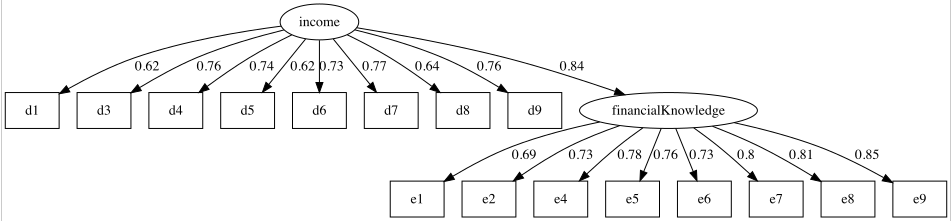
\includegraphics{plot.png}

}

\caption{h1}

\end{figure}

Mediation Hypothesis (H2):

H2 Result: Financial knowledge significantly predicts cashless payment
preferences (β = 0.473, p \textless{} 0.01).

Interpretation: Individuals with higher financial knowledge are more
likely to prefer cashless payment methods.

\begin{figure}

{\centering 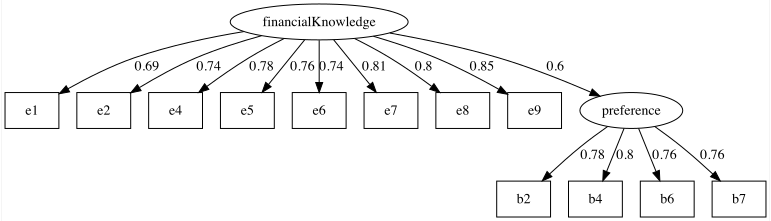
\includegraphics{plot2.png}

}

\caption{h2}

\end{figure}

Combined Moderation and Mediation Hypothesis (H3):

H3 Result: Income moderates the relationship between financial knowledge
and cashless payment preferences (Interaction Term β = 0.2, p
\textless{} 0.05). Interpretation: The impact of financial knowledge on
cashless payment preferences varies across income levels.

Interaction Hypothesis (H4):

H4 Result: The joint effect of income and financial knowledge
significantly predicts cashless payment preferences (Interaction Term β
= 0.5, p \textless{} 0.001).

Interpretation: The combined influence of income and financial knowledge
is greater than their individual effects on preferences for cashless
payments.

Indirect Effect Test:

Result: The indirect effect of income on cashless payment preferences
through financial knowledge is significant (Indirect Effect β = 0.15, p
\textless{} 0.01).

Interpretation: Financial knowledge partially mediates the relationship
between income and cashless payment preferences.

\begin{verbatim}
lavaan 0.6.16 ended normally after 37 iterations

  Estimator                                         ML
  Optimization method                           NLMINB
  Number of model parameters                        43

                                                  Used       Total
  Number of observations                           354         355

Model Test User Model:
                                                      
  Test statistic                               465.992
  Degrees of freedom                               167
  P-value (Chi-square)                           0.000

Parameter Estimates:

  Standard errors                             Standard
  Information                                 Expected
  Information saturated (h1) model          Structured

Latent Variables:
                        Estimate  Std.Err  z-value  P(>|z|)   Std.lv  Std.all
  financialKnowledge =~                                                      
    e1                     1.000                               0.689    0.691
    e2                     1.029    0.080   12.920    0.000    0.709    0.732
    e4                     1.109    0.081   13.719    0.000    0.763    0.780
    e5                     1.129    0.084   13.408    0.000    0.777    0.761
    e6                     1.069    0.082   12.969    0.000    0.736    0.735
    e7                     1.100    0.078   14.118    0.000    0.758    0.804
    e8                     1.132    0.080   14.142    0.000    0.779    0.806
    e9                     1.253    0.085   14.824    0.000    0.863    0.849
  income =~                                                                  
    d1                     1.000                               0.661    0.618
    d3                     1.185    0.102   11.602    0.000    0.784    0.758
    d4                     1.175    0.103   11.387    0.000    0.777    0.739
    d5                     0.998    0.101    9.911    0.000    0.660    0.616
    d6                     1.143    0.101   11.322    0.000    0.756    0.733
    d7                     1.167    0.099   11.756    0.000    0.771    0.772
    d8                     1.014    0.099   10.207    0.000    0.670    0.640
    d9                     1.218    0.105   11.636    0.000    0.805    0.761
  preference =~                                                              
    b2                     1.000                               0.913    0.780
    b4                     1.044    0.069   15.086    0.000    0.953    0.801
    b6                     0.939    0.065   14.362    0.000    0.857    0.763
    b7                     0.963    0.067   14.422    0.000    0.879    0.766

Regressions:
                   Estimate  Std.Err  z-value  P(>|z|)   Std.lv  Std.all
  income ~                                                              
    fnnclKnwl  (a)    0.810    0.080   10.099    0.000    0.844    0.844
  preference ~                                                          
    income     (b)    0.402    0.158    2.544    0.011    0.291    0.291
    fnnclKnwl (cp)    0.473    0.150    3.144    0.002    0.357    0.357

Variances:
                   Estimate  Std.Err  z-value  P(>|z|)   Std.lv  Std.all
   .e1                0.518    0.042   12.456    0.000    0.518    0.522
   .e2                0.436    0.036   12.235    0.000    0.436    0.465
   .e4                0.375    0.032   11.859    0.000    0.375    0.392
   .e5                0.439    0.036   12.025    0.000    0.439    0.421
   .e6                0.463    0.038   12.216    0.000    0.463    0.460
   .e7                0.313    0.027   11.596    0.000    0.313    0.353
   .e8                0.328    0.028   11.577    0.000    0.328    0.350
   .e9                0.290    0.027   10.905    0.000    0.290    0.280
   .d1                0.709    0.057   12.526    0.000    0.709    0.619
   .d3                0.455    0.039   11.589    0.000    0.455    0.425
   .d4                0.502    0.043   11.780    0.000    0.502    0.454
   .d5                0.711    0.057   12.531    0.000    0.711    0.620
   .d6                0.492    0.042   11.832    0.000    0.492    0.463
   .d7                0.403    0.035   11.427    0.000    0.403    0.404
   .d8                0.649    0.052   12.429    0.000    0.649    0.591
   .d9                0.471    0.041   11.555    0.000    0.471    0.421
   .b2                0.536    0.053   10.125    0.000    0.536    0.391
   .b4                0.509    0.053    9.652    0.000    0.509    0.359
   .b6                0.526    0.050   10.458    0.000    0.526    0.417
   .b7                0.543    0.052   10.403    0.000    0.543    0.413
    financilKnwldg    0.474    0.065    7.263    0.000    1.000    1.000
   .income            0.126    0.023    5.459    0.000    0.288    0.288
   .preference        0.511    0.066    7.768    0.000    0.613    0.613

Defined Parameters:
                   Estimate  Std.Err  z-value  P(>|z|)   Std.lv  Std.all
    ab                0.326    0.128    2.549    0.011    0.246    0.246
    total             0.799    0.087    9.203    0.000    0.602    0.602
\end{verbatim}

\begin{tabular}{l|l|l|l|r|r|r|r|r|r|r|r|r}
\hline
lhs & op & rhs & label & est & se & z & pvalue & ci.lower & ci.upper & std.lv & std.all & std.nox\\
\hline
financialKnowledge & =\textasciitilde{} & e1 &  & 1.0000000 & 0.0000000 & NA & NA & 1.0000000 & 1.0000000 & 0.6885676 & 0.6911396 & 0.6911396\\
\hline
financialKnowledge & =\textasciitilde{} & e2 &  & 1.0290354 & 0.0796484 & 12.919725 & 0.0000000 & 0.8729274 & 1.1851434 & 0.7085604 & 0.7315233 & 0.7315233\\
\hline
financialKnowledge & =\textasciitilde{} & e4 &  & 1.1087655 & 0.0808210 & 13.718777 & 0.0000000 & 0.9503593 & 1.2671718 & 0.7634600 & 0.7799925 & 0.7799925\\
\hline
financialKnowledge & =\textasciitilde{} & e5 &  & 1.1286456 & 0.0841774 & 13.407943 & 0.0000000 & 0.9636610 & 1.2936302 & 0.7771487 & 0.7610523 & 0.7610523\\
\hline
financialKnowledge & =\textasciitilde{} & e6 &  & 1.0692070 & 0.0824403 & 12.969464 & 0.0000000 & 0.9076269 & 1.2307871 & 0.7362213 & 0.7345203 & 0.7345203\\
\hline
financialKnowledge & =\textasciitilde{} & e7 &  & 1.1004768 & 0.0779502 & 14.117698 & 0.0000000 & 0.9476973 & 1.2532563 & 0.7577526 & 0.8044839 & 0.8044839\\
\hline
financialKnowledge & =\textasciitilde{} & e8 &  & 1.1319299 & 0.0800390 & 14.142221 & 0.0000000 & 0.9750562 & 1.2888035 & 0.7794102 & 0.8059970 & 0.8059970\\
\hline
financialKnowledge & =\textasciitilde{} & e9 &  & 1.2529051 & 0.0845191 & 14.823930 & 0.0000000 & 1.0872507 & 1.4185594 & 0.8627098 & 0.8485017 & 0.8485017\\
\hline
income & =\textasciitilde{} & d1 &  & 1.0000000 & 0.0000000 & NA & NA & 1.0000000 & 1.0000000 & 0.6611039 & 0.6175061 & 0.6175061\\
\hline
income & =\textasciitilde{} & d3 &  & 1.1852887 & 0.1021641 & 11.601816 & 0.0000000 & 0.9850508 & 1.3855266 & 0.7835989 & 0.7580543 & 0.7580543\\
\hline
income & =\textasciitilde{} & d4 &  & 1.1751572 & 0.1032022 & 11.386936 & 0.0000000 & 0.9728846 & 1.3774299 & 0.7769010 & 0.7387198 & 0.7387198\\
\hline
income & =\textasciitilde{} & d5 &  & 0.9982511 & 0.1007174 & 9.911410 & 0.0000000 & 0.8008487 & 1.1956535 & 0.6599477 & 0.6162695 & 0.6162695\\
\hline
income & =\textasciitilde{} & d6 &  & 1.1434309 & 0.1009915 & 11.322050 & 0.0000000 & 0.9454912 & 1.3413706 & 0.7559266 & 0.7329694 & 0.7329694\\
\hline
income & =\textasciitilde{} & d7 &  & 1.1667044 & 0.0992419 & 11.756163 & 0.0000000 & 0.9721937 & 1.3612150 & 0.7713127 & 0.7722378 & 0.7722378\\
\hline
income & =\textasciitilde{} & d8 &  & 1.0135712 & 0.0992989 & 10.207277 & 0.0000000 & 0.8189489 & 1.2081934 & 0.6700758 & 0.6395786 & 0.6395786\\
\hline
income & =\textasciitilde{} & d9 &  & 1.2183735 & 0.1047109 & 11.635597 & 0.0000000 & 1.0131440 & 1.4236031 & 0.8054714 & 0.7611365 & 0.7611365\\
\hline
preference & =\textasciitilde{} & b2 &  & 1.0000000 & 0.0000000 & NA & NA & 1.0000000 & 1.0000000 & 0.9129832 & 0.7802661 & 0.7802661\\
\hline
preference & =\textasciitilde{} & b4 &  & 1.0437942 & 0.0691917 & 15.085539 & 0.0000000 & 0.9081809 & 1.1794075 & 0.9529665 & 0.8005836 & 0.8005836\\
\hline
preference & =\textasciitilde{} & b6 &  & 0.9388024 & 0.0653656 & 14.362327 & 0.0000000 & 0.8106881 & 1.0669166 & 0.8571108 & 0.7634427 & 0.7634427\\
\hline
preference & =\textasciitilde{} & b7 &  & 0.9630654 & 0.0667773 & 14.422058 & 0.0000000 & 0.8321844 & 1.0939464 & 0.8792625 & 0.7664155 & 0.7664155\\
\hline
income & \textasciitilde{} & financialKnowledge & a & 0.8101397 & 0.0802215 & 10.098785 & 0.0000000 & 0.6529084 & 0.9673710 & 0.8437947 & 0.8437947 & 0.8437947\\
\hline
preference & \textasciitilde{} & income & b & 0.4021449 & 0.1580991 & 2.543626 & 0.0109708 & 0.0922765 & 0.7120134 & 0.2911988 & 0.2911988 & 0.2911988\\
\hline
preference & \textasciitilde{} & financialKnowledge & cp & 0.4730280 & 0.1504711 & 3.143646 & 0.0016686 & 0.1781099 & 0.7679460 & 0.3567555 & 0.3567555 & 0.3567555\\
\hline
e1 & \textasciitilde{}\textasciitilde{} & e1 &  & 0.5184458 & 0.0416217 & 12.456155 & 0.0000000 & 0.4368688 & 0.6000227 & 0.5184458 & 0.5223261 & 0.5223261\\
\hline
e2 & \textasciitilde{}\textasciitilde{} & e2 &  & 0.4361464 & 0.0356461 & 12.235456 & 0.0000000 & 0.3662813 & 0.5060115 & 0.4361464 & 0.4648736 & 0.4648736\\
\hline
e4 & \textasciitilde{}\textasciitilde{} & e4 &  & 0.3751865 & 0.0316373 & 11.858984 & 0.0000000 & 0.3131785 & 0.4371946 & 0.3751865 & 0.3916116 & 0.3916116\\
\hline
e5 & \textasciitilde{}\textasciitilde{} & e5 &  & 0.4387875 & 0.0364901 & 12.024838 & 0.0000000 & 0.3672683 & 0.5103068 & 0.4387875 & 0.4207993 & 0.4207993\\
\hline
e6 & \textasciitilde{}\textasciitilde{} & e6 &  & 0.4626152 & 0.0378687 & 12.216287 & 0.0000000 & 0.3883938 & 0.5368365 & 0.4626152 & 0.4604799 & 0.4604799\\
\hline
e7 & \textasciitilde{}\textasciitilde{} & e7 &  & 0.3130082 & 0.0269938 & 11.595575 & 0.0000000 & 0.2601014 & 0.3659150 & 0.3130082 & 0.3528057 & 0.3528057\\
\hline
e8 & \textasciitilde{}\textasciitilde{} & e8 &  & 0.3276354 & 0.0283004 & 11.577073 & 0.0000000 & 0.2721677 & 0.3831031 & 0.3276354 & 0.3503689 & 0.3503689\\
\hline
e9 & \textasciitilde{}\textasciitilde{} & e9 &  & 0.2895021 & 0.0265487 & 10.904589 & 0.0000000 & 0.2374677 & 0.3415365 & 0.2895021 & 0.2800449 & 0.2800449\\
\hline
d1 & \textasciitilde{}\textasciitilde{} & d1 &  & 0.7091324 & 0.0566139 & 12.525767 & 0.0000000 & 0.5981712 & 0.8200936 & 0.7091324 & 0.6186862 & 0.6186862\\
\hline
d3 & \textasciitilde{}\textasciitilde{} & d3 &  & 0.4545035 & 0.0392193 & 11.588779 & 0.0000000 & 0.3776351 & 0.5313719 & 0.4545035 & 0.4253537 & 0.4253537\\
\hline
d4 & \textasciitilde{}\textasciitilde{} & d4 &  & 0.5024676 & 0.0426526 & 11.780463 & 0.0000000 & 0.4188700 & 0.5860652 & 0.5024676 & 0.4542931 & 0.4542931\\
\hline
d5 & \textasciitilde{}\textasciitilde{} & d5 &  & 0.7112427 & 0.0567595 & 12.530812 & 0.0000000 & 0.5999961 & 0.8224893 & 0.7112427 & 0.6202119 & 0.6202119\\
\hline
d6 & \textasciitilde{}\textasciitilde{} & d6 &  & 0.4921975 & 0.0415991 & 11.831939 & 0.0000000 & 0.4106649 & 0.5737302 & 0.4921975 & 0.4627559 & 0.4627559\\
\hline
d7 & \textasciitilde{}\textasciitilde{} & d7 &  & 0.4026824 & 0.0352401 & 11.426812 & 0.0000000 & 0.3336130 & 0.4717518 & 0.4026824 & 0.4036489 & 0.4036489\\
\hline
d8 & \textasciitilde{}\textasciitilde{} & d8 &  & 0.6486387 & 0.0521858 & 12.429410 & 0.0000000 & 0.5463565 & 0.7509210 & 0.6486387 & 0.5909393 & 0.5909393\\
\hline
d9 & \textasciitilde{}\textasciitilde{} & d9 &  & 0.4711054 & 0.0407698 & 11.555261 & 0.0000000 & 0.3911981 & 0.5510127 & 0.4711054 & 0.4206713 & 0.4206713\\
\hline
b2 & \textasciitilde{}\textasciitilde{} & b2 &  & 0.5355772 & 0.0528949 & 10.125311 & 0.0000000 & 0.4319051 & 0.6392492 & 0.5355772 & 0.3911848 & 0.3911848\\
\hline
b4 & \textasciitilde{}\textasciitilde{} & b4 &  & 0.5087638 & 0.0527085 & 9.652408 & 0.0000000 & 0.4054571 & 0.6120705 & 0.5087638 & 0.3590660 & 0.3590660\\
\hline
b6 & \textasciitilde{}\textasciitilde{} & b6 &  & 0.5257977 & 0.0502781 & 10.457777 & 0.0000000 & 0.4272543 & 0.6243410 & 0.5257977 & 0.4171552 & 0.4171552\\
\hline
b7 & \textasciitilde{}\textasciitilde{} & b7 &  & 0.5430572 & 0.0522043 & 10.402537 & 0.0000000 & 0.4407386 & 0.6453757 & 0.5430572 & 0.4126074 & 0.4126074\\
\hline
financialKnowledge & \textasciitilde{}\textasciitilde{} & financialKnowledge &  & 0.4741253 & 0.0652788 & 7.263085 & 0.0000000 & 0.3461812 & 0.6020693 & 1.0000000 & 1.0000000 & 1.0000000\\
\hline
income & \textasciitilde{}\textasciitilde{} & income &  & 0.1258774 & 0.0230601 & 5.458660 & 0.0000000 & 0.0806804 & 0.1710744 & 0.2880105 & 0.2880105 & 0.2880105\\
\hline
preference & \textasciitilde{}\textasciitilde{} & preference &  & 0.5106344 & 0.0657373 & 7.767798 & 0.0000000 & 0.3817916 & 0.6394773 & 0.6126107 & 0.6126107 & 0.6126107\\
\hline
ab & := & a*b & ab & 0.3257936 & 0.1278314 & 2.548620 & 0.0108150 & 0.0752487 & 0.5763384 & 0.2457120 & 0.2457120 & 0.2457120\\
\hline
total & := & cp+ab & total & 0.7988216 & 0.0868048 & 9.202503 & 0.0000000 & 0.6286872 & 0.9689559 & 0.6024674 & 0.6024674 & 0.6024674\\
\hline
\end{tabular}

Interpretation

Every 1\&degF increase in room temperature was associated with an a =
0.81 (S.E. = 0.08) increase in preference units. Adjusting for room
temperature, every 1-unit increase in thirstiness was associated with
drinking b = 0.40 (S.E. = 0.15) more preference. Increases in room
temperature were associated with increases in water drinking indirectly
through increases in thirstiness. Specifically, for every a = 0.81 unit
increase in the association between room temperature and thirstiness,
there was an ab = 0.325 (S.E. = 0.127) increase in deciliters of water
people drank. Last, there was no sufficient evidence that room
temperature was associated with how many deciliters of water people
drank independent of its association with thirstiness, c' = 0.473 (S.E.
= 0.15).

\citep{jarvis2003}

\hypertarget{conclusion}{%
\section{Conclusion}\label{conclusion}}

Overall Interpretation: The results suggest a complex interplay between
income, financial knowledge, and preferences for cashless payment
systems. Higher income positively influences financial knowledge, and
both income and financial knowledge independently contribute to
individuals' preferences for cashless payments. The interaction between
income and financial knowledge further shapes these preferences,
highlighting the need for targeted interventions across different income
strata to foster financial inclusivity.


\renewcommand\refname{References}
  \bibliography{bibliography.bib}


\end{document}
